\subsection{Relaxation Eligibility and Measured Cost}
\begin{figure*}[t]
\centering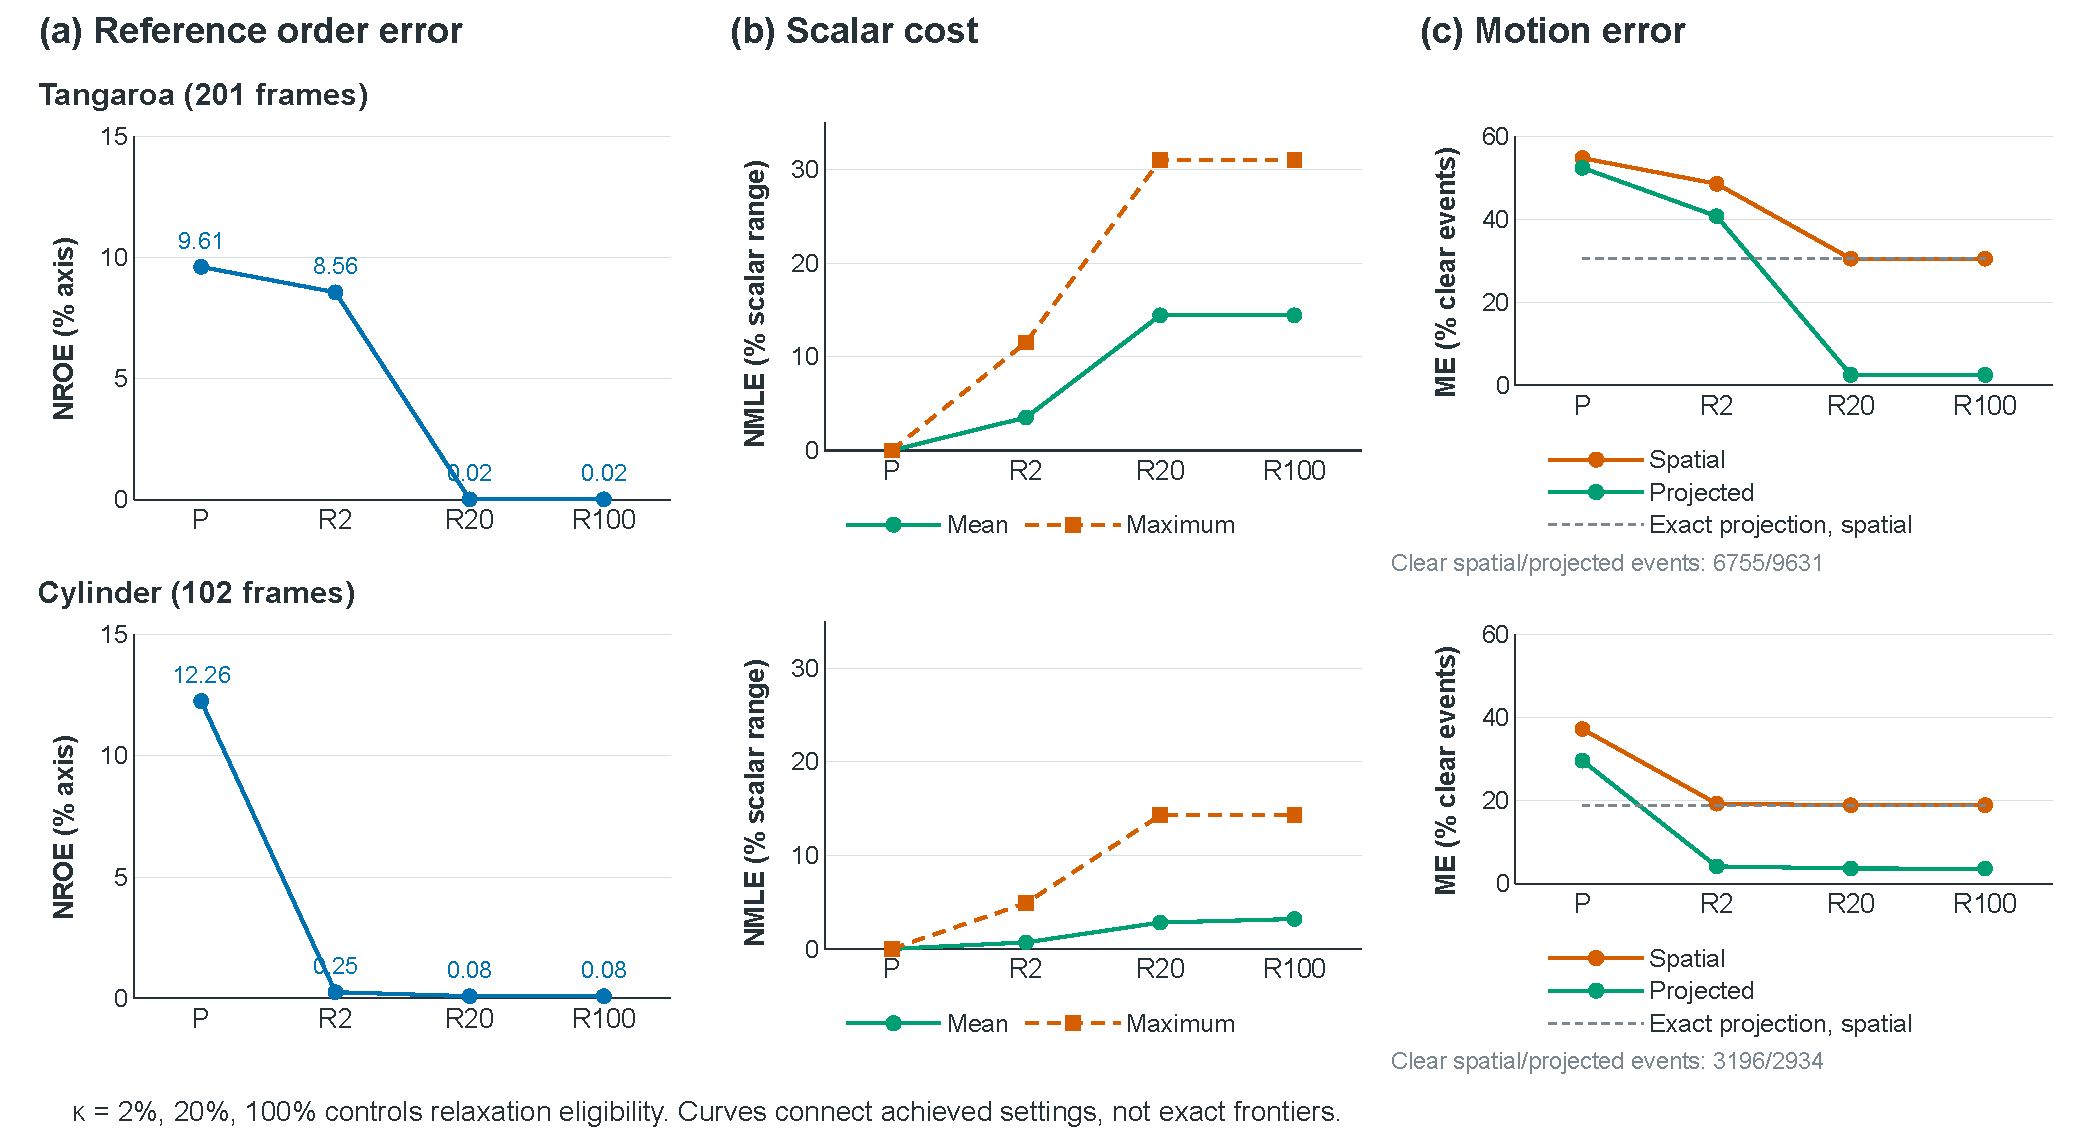
\includegraphics[width=\textwidth]{figures/Fig14.pdf}
\caption{Eligibility and measured position--scalar trade-offs on Tangaroa and Cylinder. Saved P, R2, R20, and R100 outputs share each dataset's source fields and persistence. NROE and NMLE are independently measured; $\kappa$ selects eligible parent gaps rather than capping output error. Larger settings need not improve both quantities: Tangaroa R20/R100 coincide, while Cylinder R100 matches R20's order error with greater mean scalar cost. These large-tree operating points do not form an exhaustive exact frontier.}
\label{fig:eligibility_tradeoff}
\end{figure*}

Figure~\ref{fig:eligibility_tradeoff} compares P, R2, R20 and R100 on the same complete Tangaroa and Cylinder inputs. The threshold $\kappa$ selects eligible parent gaps; it is not a bound on the measured output NMLE. Tangaroa R20 and R100 coincide. Cylinder R100 retains R20's mean NROE while increasing mean NMLE from 2.810\% to 3.190\%. The grey exact-projection reference uses its own clear-event population and supplies a diagnostic, rather than a universal lower bound on spatial-motion error. These operating points complement the exhaustive small-tree frontiers without claiming exhaustive enumeration for the larger trees.
